% Options for packages loaded elsewhere
\PassOptionsToPackage{unicode}{hyperref}
\PassOptionsToPackage{hyphens}{url}
\PassOptionsToPackage{dvipsnames,svgnames*,x11names*}{xcolor}
%
\documentclass[
  ngerman,
  a4paper,
  12pt]{scrartcl}
\usepackage{lmodern}
\usepackage{amssymb,amsmath}
\usepackage{ifxetex,ifluatex}
\ifnum 0\ifxetex 1\fi\ifluatex 1\fi=0 % if pdftex
  \usepackage[T1]{fontenc}
  \usepackage[utf8]{inputenc}
  \usepackage{textcomp} % provide euro and other symbols
\else % if luatex or xetex
  \usepackage{unicode-math}
  \defaultfontfeatures{Scale=MatchLowercase}
  \defaultfontfeatures[\rmfamily]{Ligatures=TeX,Scale=1}
\fi
% Use upquote if available, for straight quotes in verbatim environments
\IfFileExists{upquote.sty}{\usepackage{upquote}}{}
\IfFileExists{microtype.sty}{% use microtype if available
  \usepackage[]{microtype}
  \UseMicrotypeSet[protrusion]{basicmath} % disable protrusion for tt fonts
}{}
\makeatletter
\@ifundefined{KOMAClassName}{% if non-KOMA class
  \IfFileExists{parskip.sty}{%
    \usepackage{parskip}
  }{% else
    \setlength{\parindent}{0pt}
    \setlength{\parskip}{6pt plus 2pt minus 1pt}}
}{% if KOMA class
  \KOMAoptions{parskip=half}}
\makeatother
\usepackage{xcolor}
\IfFileExists{xurl.sty}{\usepackage{xurl}}{} % add URL line breaks if available
\IfFileExists{bookmark.sty}{\usepackage{bookmark}}{\usepackage{hyperref}}
\hypersetup{
  pdftitle={Steuerung eines Arduino Uno Mikrokontrollers via WebSocket},
  pdfauthor={Samuel Hess},
  pdflang={de},
  pdfsubject={ICT Modul 121 - Steuerungsaufgaben bearbeiten},
  colorlinks=true,
  linkcolor=Maroon,
  filecolor=Maroon,
  citecolor=Blue,
  urlcolor=blue,
  pdfcreator={LaTeX via pandoc}}
\urlstyle{same} % disable monospaced font for URLs
\usepackage{graphicx}
\makeatletter
\def\maxwidth{\ifdim\Gin@nat@width>\linewidth\linewidth\else\Gin@nat@width\fi}
\def\maxheight{\ifdim\Gin@nat@height>\textheight\textheight\else\Gin@nat@height\fi}
\makeatother
% Scale images if necessary, so that they will not overflow the page
% margins by default, and it is still possible to overwrite the defaults
% using explicit options in \includegraphics[width, height, ...]{}
\setkeys{Gin}{width=\maxwidth,height=\maxheight,keepaspectratio}
% Set default figure placement to htbp
\makeatletter
\def\fps@figure{htbp}
\makeatother
\setlength{\emergencystretch}{3em} % prevent overfull lines
\providecommand{\tightlist}{%
  \setlength{\itemsep}{0pt}\setlength{\parskip}{0pt}}
\setcounter{secnumdepth}{5}
\ifxetex
  % Load polyglossia as late as possible: uses bidi with RTL langages (e.g. Hebrew, Arabic)
  \usepackage{polyglossia}
  \setmainlanguage[]{german}
\else
  \usepackage[shorthands=off,main=ngerman]{babel}
\fi
\newlength{\cslhangindent}
\setlength{\cslhangindent}{1.5em}
\newenvironment{cslreferences}%
  {\setlength{\parindent}{0pt}%
  \everypar{\setlength{\hangindent}{\cslhangindent}}\ignorespaces}%
  {\par}

\title{Steuerung eines Arduino Uno Mikrokontrollers via WebSocket}
\author{Samuel Hess}
\date{12. Mai 2020}

\begin{document}
\maketitle

\renewcommand*\contentsname{Inhaltsverzeichnis}
{
\hypersetup{linkcolor=}
\setcounter{tocdepth}{2}
\tableofcontents
}
\hypertarget{abstract}{%
\section{Abstract}\label{abstract}}

In der vorliegenden Arbeit wurde untersucht, wie ein Arduino Uno über
eine WebSocket-Verbindung gesteuert werden kann, während dieser im
Sekundentakt Statusmeldungen versendet.

Der verwendete Funduino Uno R3 {[}\protect\hyperlink{ref-lernset}{1}{]}
verfügt über keine WLAN-Schnittstelle. Daher erfolgt die
WebSocket-Kommunikation extern auf einem Gateway. Als Gateway wird ein
Windows-PC verwendet. Arduino und Gateway sind per USB verbunden und
kommunizieren über eine virtuelle serielle Schnittstelle.

Das Ergebnis zeigt, dass eine Steuerung eines Arduinos per WebSocket
problemlos möglich ist. Die eingehenden Nachrichten müssen auf dem
Arduino geparst werden. Dieses Parding ist einfacher, wenn das
verwendete Austauschformt schlank gehalten wird. Deshalb wurde anstelle
von JSON das URL Format verwendet.

\hypertarget{einleitung}{%
\section{Einleitung}\label{einleitung}}

In diesem Kapitel wird die Motivation erläutert und genaue Fragesellung
definiert. Dann folgt eine kleine Übersichtsarbeit mit dazugehöriger
Literaturrecherche.

\hypertarget{fragestellung}{%
\subsection{Fragestellung}\label{fragestellung}}

Welche Möglichkeiten gibt es, einen Arduino Uno via Websocket zu
steuern?

Während einer explorativen Online-Suche wurden einzelne Lösungen
gefunden. Eine systematische Zusammenstellung der Möglichkeiten fehlt
jedoch.

\hypertarget{motivation}{%
\subsection{Motivation}\label{motivation}}

Die Motivation für die vorliegende Arbeit ist die Beantwortung der
nachfolgenden Fragestellung. Weiter soll der Artikel interessierten
Lesern als Einstiegslektüre diesen.

\hypertarget{literatur-review}{%
\subsection{Literatur-Review}\label{literatur-review}}

Zum Thema existiert diverse Fachliteratur unter anderem von Erik
Bartmann {[}\protect\hyperlink{ref-bartmannArduino}{2}{]}
{[}\protect\hyperlink{ref-bartmannESP8266}{3}{]}
{[}\protect\hyperlink{ref-bartmannESP32}{4}{]}.

\hypertarget{arduino-mit-integriertem-wlan}{%
\subsubsection{Arduino mit integriertem
WLAN}\label{arduino-mit-integriertem-wlan}}

Der Arduino Uno hat keine eingebaute WLAN Schnittstelle. Es gibt jedoch
andere Arduino Modelle mit integriertem WLAN, wie z.B. der Arduino
MKR1000.

\hypertarget{wlan-erweiterung}{%
\subsubsection{WLAN Erweiterung}\label{wlan-erweiterung}}

Mehrere Autoren berichten
{[}\protect\hyperlink{ref-temperatureDashboard}{5}{]}
{[}\protect\hyperlink{ref-websocketcommunication}{6}{]}, wie der Arduino
mit dem dem WLAN Modul ESP8266 erweitert werden kann.

\hypertarget{serial-gateway}{%
\subsubsection{Serial Gateway}\label{serial-gateway}}

Eine weitere Möglichkeit, ist behelfsweise einen PC als Serial Gateway
einzusetzen. Mangels kurzfristig verfügbarer Hardware wollen wir diese
Option verfolgen.

\hypertarget{experimenteller-teil}{%
\section{Experimenteller Teil}\label{experimenteller-teil}}

\hypertarget{informationsquellen}{%
\subsection{Informationsquellen}\label{informationsquellen}}

Als Informationsquellen sind die Datenblätter zur jweiligen Hardware
sowie die Manuals zu den einsesetzten Softwarekomponenten zu nennen.

\hypertarget{prinzipskizze}{%
\subsection{Prinzipskizze}\label{prinzipskizze}}

\begin{figure}
\centering
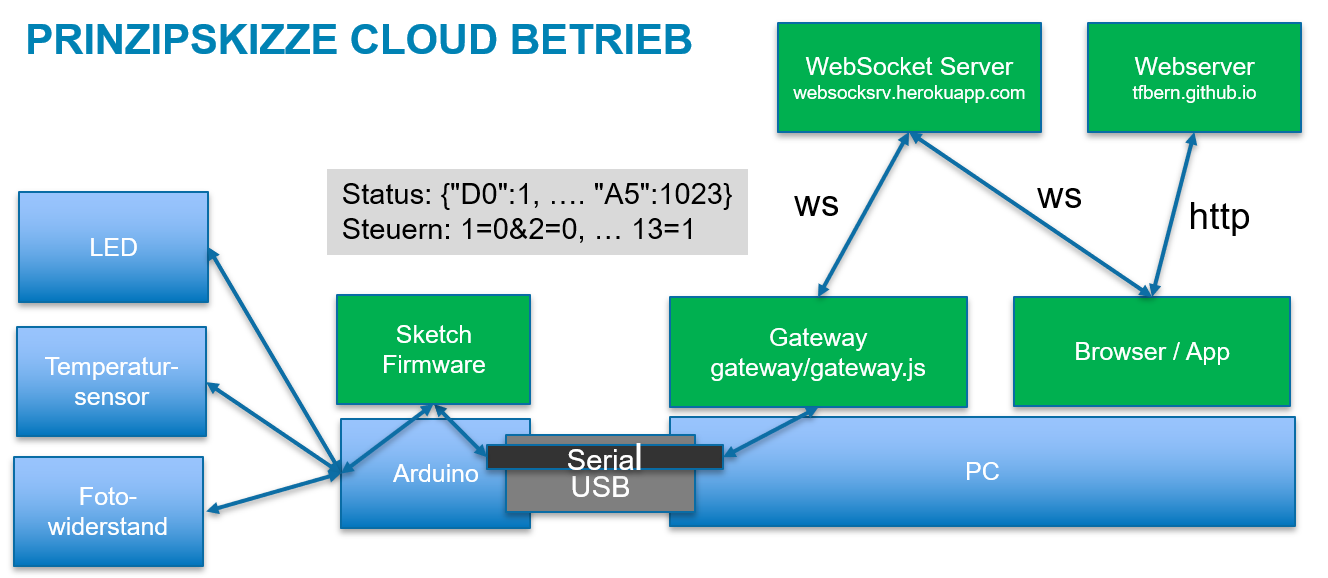
\includegraphics{img/prinzipskizze.png}
\caption{Prinzipskizze}
\end{figure}

\hypertarget{hardware}{%
\subsection{Hardware}\label{hardware}}

Verwendet wurde das Lernset Nr. 8 von Funduino
{[}\protect\hyperlink{ref-lernset}{1}{]}. Darin enthalten ist ein
Funduino Uno. Weiter benötigen wir den Temparatursensor TMP36 und den
Fotowiderstand.

\hypertarget{anschluss-der-sensoren}{%
\subsubsection{Anschluss der Sensoren}\label{anschluss-der-sensoren}}

\begin{figure}
\centering
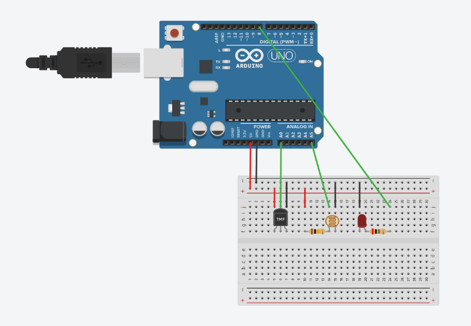
\includegraphics{img/anschluss.png}
\caption{Anschluss der Sensoren}
\end{figure}

\hypertarget{software}{%
\subsection{Software}\label{software}}

\hypertarget{entwicklungsumgebung}{%
\subsubsection{Entwicklungsumgebung}\label{entwicklungsumgebung}}

Zur Entwicklung wurde folgende Software eingesetzt.

\begin{itemize}
\tightlist
\item
  Visual Studio Code {[}\protect\hyperlink{ref-vscode}{7}{]} mit der
  Erweiterung C/C++ IntelliSense
  {[}\protect\hyperlink{ref-intellisense}{8}{]}
\item
  Arduino CLI {[}\protect\hyperlink{ref-arduinoCli}{9}{]}
\item
  Git for Windows {[}\protect\hyperlink{ref-gitForWindows}{10}{]} und
  TortoiseGit {[}\protect\hyperlink{ref-tortoiseGit}{11}{]}
\end{itemize}

Nicht verwendet wurde die Arduino IDE. Windows verwendet den
Standardtreiber \emph{usbser.sys} für den virtuellen COM Port.

\hypertarget{node-libraries}{%
\subsubsection{Node Libraries}\label{node-libraries}}

Weiter wurde folgende NPM Packages eingesetzt:

\begin{itemize}
\tightlist
\item
  WebSockets {[}\protect\hyperlink{ref-websockets}{12}{]}
\item
  Express {[}\protect\hyperlink{ref-express}{13}{]}
\item
  Chart.js {[}\protect\hyperlink{ref-chartjs}{14}{]}
\item
  SerialPort {[}\protect\hyperlink{ref-serialPort}{15}{]}
\end{itemize}

\hypertarget{arduino-libraries}{%
\subsubsection{Arduino Libraries}\label{arduino-libraries}}

Weiter wurde folgende Arduino Libraries eingesetzt:

\begin{itemize}
\tightlist
\item
  Arduino Library (Arduino.h)
  {[}\protect\hyperlink{ref-sprachreferenz}{16}{]}
  {[}\protect\hyperlink{ref-codeReferenz}{17}{]}
  {[}\protect\hyperlink{ref-arduinoCheatSheet}{18}{]}\\
\item
  AVR Libc {[}\protect\hyperlink{ref-avrlibc}{19}{]}
\end{itemize}

\hypertarget{arduino-sketch}{%
\subsubsection{Arduino Sketch}\label{arduino-sketch}}

Zunächst müssen wir klären, in welcher Programmiersprache die Arduino
Sketches geschrieben werden. Nachdem man sich die Build-Umgebung genauer
unter die Lupe genommen hat, wird klar, dass keine eigene
Arduino-Sprache
existiert{[}\protect\hyperlink{ref-arduinoLanguage}{20}{]}. Im
Hintergrund wird aus dem Sketch eine C++ Datei erstellt und mit
\emph{avr-g++} kompiliert.

Die Problematik der Heap-Fragmentierung wird von mehreren Autoren
aufgeworfen und diskutiert
{[}\protect\hyperlink{ref-heapFragmentation}{21}{]}{[}\protect\hyperlink{ref-heapFragmentation2}{22}{]}.
Matt ist der Meinung, dass man deshalb auf die String Klasse in der
Arduino Library gänzlich verzichten soll
{[}\protect\hyperlink{ref-arduinoStrings}{23}{]}. In der Konsequenz
müsste man die Stringfunktion aus der Standard C Library
{[}\protect\hyperlink{ref-avrlibc}{19}{]} verwenden und in C
programmieren. Ich sehe dies nicht ganz so eng und setze die Arduino
String Klasse trotzdem, jedoch mit Zurückhaltung ein. Ich befolge Matt's
Rat, die Variablen by Reference zu übergeben
{[}\protect\hyperlink{ref-arduinoStrings}{23}{]}.

Der Quellcode befindet sich im Ordner Arduino. Darin befinden sich
verschiedene Sketech, darunter
\href{../../arduino/genericReadWrite/genericReadWrite.ino}{genericReadWrite}

\hypertarget{serial-gateway-1}{%
\subsubsection{Serial Gateway}\label{serial-gateway-1}}

Der Quellcode befindet sich im Ordner
\href{../../gateway/gateway.js}{Gateway}.

\hypertarget{websocket-server}{%
\subsubsection{WebSocket Server}\label{websocket-server}}

Der Quellcode befindet sich im Ordner
\href{../../websocketserver/websocketserver.js}{WebSocketServer}.

\hypertarget{web-gui}{%
\subsubsection{Web GUI}\label{web-gui}}

Der Quellcode befindet sich im Ordner
\href{../../client/index.html}{Client}.

\hypertarget{resultate}{%
\section{Resultate}\label{resultate}}

Es hat sich gezeigt, dass ein Seriell-zu-Websocket-Gatway unter Node.js
einfach zu implementieren ist. Über diesen Umweg kann der Arduino Uno
ans Internet angebunden werden.

\hypertarget{diskussion}{%
\section{Diskussion}\label{diskussion}}

\hypertarget{zusammenfassung}{%
\section{Zusammenfassung}\label{zusammenfassung}}

Statt des Arduino Uno könnte ein Arduino MKR1000 verwendet werden.
Dieser könnte kann auch an die Arduino Clound angebunden werden. Ein
weitere Option ist die Beschaffung einer WLAN Erweiterung wie das Modul
ESP8266.

\hypertarget{danksagung}{%
\section{Danksagung}\label{danksagung}}

Ich danke den Lernenden der Klasse BINF2017A für die Zusammenarbeit.

\hypertarget{interessenskonflikte}{%
\section{Interessenskonflikte}\label{interessenskonflikte}}

Das Projekt wurde im Rahmen des Beruffachschulunterrichts durchgeführt
und erhielt keine externde Finanzierung. Demnach bestehen keien
Interessenkonflikte.

\hypertarget{quellenverzeichnis}{%
\section*{Quellenverzeichnis}\label{quellenverzeichnis}}
\addcontentsline{toc}{section}{Quellenverzeichnis}

\hypertarget{refs}{}
\begin{cslreferences}
\leavevmode\hypertarget{ref-lernset}{}%
{[}1{]} \emph{Lernset Nr.8 mit UNO Controller - Kit für Arduino}. URL
\url{https://www.funduinoshop.com/epages/78096195.sf/de_DE/?ObjectPath=/Shops/78096195/Products/01-U8}

\leavevmode\hypertarget{ref-bartmannArduino}{}%
{[}2{]} \textsc{Bartmann, Erik}: \emph{Mit Arduino die elektronische
Welt entdecken}. 3. Aufl.~: Bombini-Verlag, 2017
---~ISBN~\href{https://worldcat.org/isbn/978-3-946496-00-7}{978-3-946496-00-7}

\leavevmode\hypertarget{ref-bartmannESP8266}{}%
{[}3{]} \textsc{Bartmann, Erik}: \emph{Das ESP8266-Praxisbuch: Mit
NodeMCU und ESPlorer}~: Elektor Verlag, 2016
---~ISBN~\href{https://worldcat.org/isbn/978-3-89576-321-2}{978-3-89576-321-2}

\leavevmode\hypertarget{ref-bartmannESP32}{}%
{[}4{]} \textsc{Bartmann, Erik}: \emph{Das ESP32-Praxisbuch:
Programmieren mit der Arduino-IDE}~: Elektor Verlag, 2018
---~ISBN~\href{https://worldcat.org/isbn/978-3-89576-333-5}{978-3-89576-333-5}

\leavevmode\hypertarget{ref-temperatureDashboard}{}%
{[}5{]} \textsc{Andrew Shvayka, Igor Khanenko, \textnormal{Igor
Kulikov}}: \emph{Temperature Dashboard Using Arduino UNO, ESP8266 And
MQTT}. URL
\url{https://www.hackster.io/thingsboard/temperature-dashboard-using-arduino-uno-esp8266-and-mqtt-5e26eb}

\leavevmode\hypertarget{ref-websocketcommunication}{}%
{[}6{]} \emph{WebSocket communication with an ESP8266 or Arduino in
Python. Test with the ws4py library on Raspberry Pi}. URL
\url{https://diyprojects.io/websocket-communication-esp8266-arduino-python-test-ws4py-library-raspberry-pi/\#.Xq6bKagzaUk}

\leavevmode\hypertarget{ref-vscode}{}%
{[}7{]} \emph{Visual Studio Code}. URL
\url{https://code.visualstudio.com/}

\leavevmode\hypertarget{ref-intellisense}{}%
{[}8{]} \emph{C/C++ IntelliSense, debugging, and code browsing.} URL
\url{https://marketplace.visualstudio.com/items?itemName=ms-vscode.cpptools}

\leavevmode\hypertarget{ref-arduinoCli}{}%
{[}9{]} \emph{Arduino CLI}. URL
\url{https://github.com/arduino/arduino-cli}

\leavevmode\hypertarget{ref-gitForWindows}{}%
{[}10{]} \emph{Git for Windows}. URL \url{https://gitforwindows.org}

\leavevmode\hypertarget{ref-tortoiseGit}{}%
{[}11{]} \emph{TortoiseGit}. URL \url{https://tortoisegit.org}

\leavevmode\hypertarget{ref-websockets}{}%
{[}12{]} \emph{Simple to use, blazing fast and thoroughly tested
WebSocket client and server for Node.js}. URL
\url{https://github.com/websockets/ws}

\leavevmode\hypertarget{ref-express}{}%
{[}13{]} \emph{Express Schnelles, offenes, unkompliziertes Web-Framework
für Node.js}. URL \url{https://expressjs.com}

\leavevmode\hypertarget{ref-chartjs}{}%
{[}14{]} \emph{Simple yet flexible JavaScript charting for designers \&
developers}. URL \url{https://www.chartjs.org}

\leavevmode\hypertarget{ref-serialPort}{}%
{[}15{]} \emph{Node SerialPort}. URL \url{https://serialport.io}

\leavevmode\hypertarget{ref-sprachreferenz}{}%
{[}16{]} \emph{Sprach-Referenz}. URL
\url{https://www.arduino.cc/reference/de/}

\leavevmode\hypertarget{ref-codeReferenz}{}%
{[}17{]} \emph{Arduino Befehlsübersicht}. URL
\url{https://www.arduinoforum.de/code-referenz}

\leavevmode\hypertarget{ref-arduinoCheatSheet}{}%
{[}18{]} \emph{Arduino Programming Cheat Sheet}. URL
\url{https://github.com/liffiton/Arduino-Cheat-Sheet}

\leavevmode\hypertarget{ref-avrlibc}{}%
{[}19{]} \emph{AVR Libc}. URL \url{https://www.nongnu.org/avr-libc/}

\leavevmode\hypertarget{ref-arduinoLanguage}{}%
{[}20{]} \emph{C++ vs. The Arduino Language?} URL
\url{https://arduino.stackexchange.com/questions/816/c-vs-the-arduino-language}

\leavevmode\hypertarget{ref-heapFragmentation}{}%
{[}21{]} \emph{What is Heap Fragmentation?} URL
\url{https://cpp4arduino.com/2018/11/06/what-is-heap-fragmentation.html}

\leavevmode\hypertarget{ref-heapFragmentation2}{}%
{[}22{]} \textsc{Walls, Colin}: \emph{Dynamic Memory Allocation and
Fragmentation in C and C++}. URL
\url{https://www.design-reuse.com/articles/25090/dynamic-memory-allocation-fragmentation-c.html}

\leavevmode\hypertarget{ref-arduinoStrings}{}%
{[}23{]} \emph{The Evils of Arduino Strings}. URL
\url{https://majenko.co.uk/blog/evils-arduino-strings}
\end{cslreferences}

\end{document}
